\makeatletter\let\ifGm@compatii\relax\makeatother
\documentclass{beamer}
\usetheme{Warsaw}
\useoutertheme{infolines}
\setbeamertemplate{headline}[default]
\usepackage{lmodern}
\usepackage{moreverb}
\usepackage{amsmath}
\usepackage{amsfonts}
\usepackage{amssymb}
\usepackage{textcomp}
\usepackage{pifont}

%\setbeamercovered{transparent}
%\setbeamertemplate{footline}[default]
%\setbeamertemplate{headline}[split]
\usepackage[utf8]{inputenc}
%\usepackage[francais]{babel}
\usepackage{color}  

\usepackage{multicol}

% input of the tilte
% =============== 
% set of variables 
% ===============

% the title
\def\presentation{PER PROJECT DEFENCE}
\def\bottomTitle{PER PROJECT}
\def\noteAboutAuthor{Engeneering students/ENSEIRB-MATMECA}
\def\subject{Grid deformation for data visualization}
%\def\subject{Déformation de Grille pour la visualisation d'information}
% =================
% Header
% =================
\title[\bottomTitle]{
        {\bfseries \huge \presentation\\} 
        {\bfseries \subject}\\
        {\small\bf A. Lambert, R. Bourqui, D. Auber}\\   
}

\titlegraphic{
  
\includegraphics[scale=0.15]{../rapport/img/logobordeaux1.jpg}
  \hspace{2cm}
  
\includegraphics[scale=0.25]{../rapport/img/noms.png}
  \hspace{2cm}
  
\includegraphics[scale=0.25]{../rapport/img/logo.jpg}
}

\author[\noteAboutAuthor]{
  {\normalsize \bfseries \sffamily Clients : }
  David {\sc Auber} \hspace{1cm} Romain {\sc Bourqui}\\    
}



\begin{document}

%%%% Page de titre %%%%
\begin{frame}
\titlepage
\end{frame}


\begin{frame}{Plan}
  \tableofcontents[hideallsubsections]
\end{frame}

% ===============
% Les actions
% ===============

\AtBeginSection[]{
  \begin{frame}{Contents}
  \tableofcontents[currentsection,hideallsubsections]
  \end{frame}
}

\AtBeginSubsection[]{
  \begin{frame}{Contents}
  \tableofcontents[currentsection,currentsubsection]
  \end{frame}
}

% ===============
% Le plan
% ===============               
\section{Introduction}
\chapter*{Introduction}

The article summarized in this document was written by A.Lambert, R.Bourqui and D . Auber, researchers in LaBRI in Bordeaux.


This article speaks about how to visualize graphs containing many nodes and edges. With improvements in data acquisition comes an increase of the size and the complexity of graphs and this huge amount of data generally causes visual clutter, in our case due to edges crossing.
For example, it could be interesting to visualize data in fields like biology, social sciences, data mining or computer science and then emphasize their high-level pattern to help users perceive underlying models.


Nowadays, in the research world, the information is easily represented into graphs to visualize more and more data. However, this huge amount of information prevents the graph from being manually drawn:  It explains the need of software able to generate an appropriate graph with all nodes and edges. Yet this graph may suffer from cluttering, which should be reduced for a better understanding.


The first part of this document presents review related work on reducing edge clutters and enhancing edge bundles visualization, with which the article is connected. The second will deal with the Tutte algorithm , followed by the implementation issues. A third part will show our results. Finally, we draw a conclusion and explain the limits of our work for further improvements.


\section{The context}
\frame{
  \frametitle{The context}
\begin{center} 
Easy understanding with effective representation
 \end{center}
  \begin{figure}[H]
    \centering
    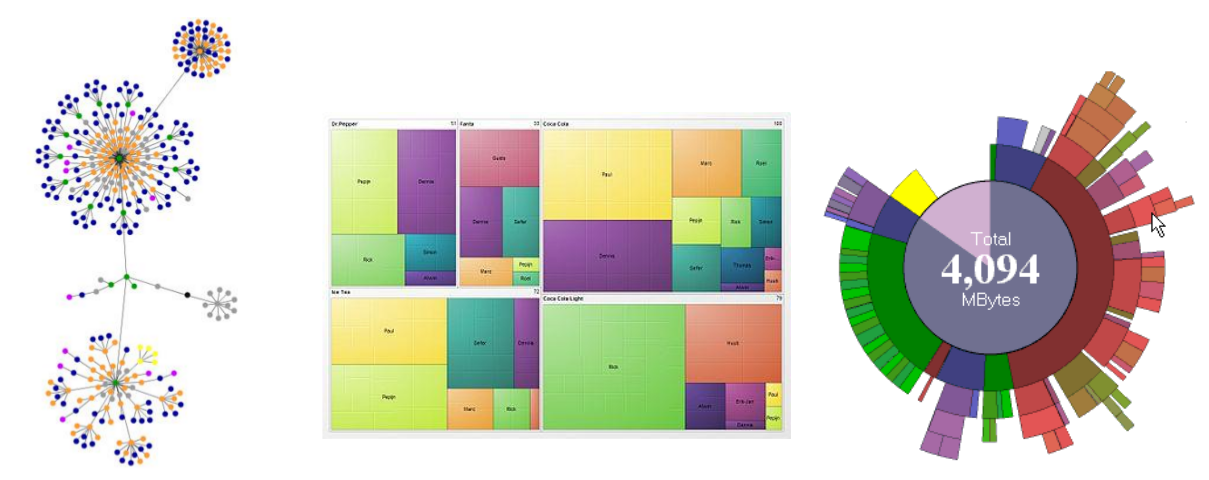
\includegraphics[scale=0.29]{../rapport/img/graphes_jolis.png}
  \end{figure}
  \pause
  \begin{alertblock}{}
    Only available for few graphs
\end{alertblock}
\vspace{1cm}
} 

\frame{
  \frametitle{The context}
  \framesubtitle{Two different methods}
  \begin{figure}[H]
    \centering
    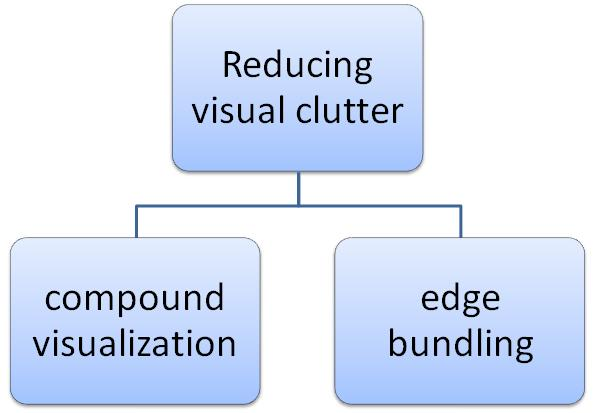
\includegraphics[scale=0.4]{../rapport/img/slide3.jpg}
  \end{figure}
 
\vspace{1cm}
} 

\frame{
  \frametitle{The context}
  \framesubtitle{Compound visualization}
  \begin{figure}[H]
    \centering
    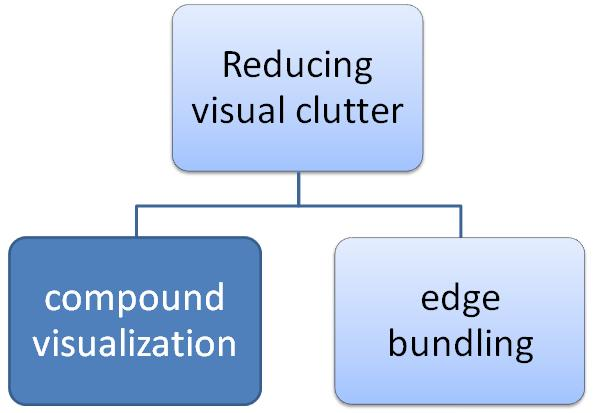
\includegraphics[scale=0.4]{../rapport/img/slide4.jpg}
  \end{figure}
 
\vspace{1cm}
} 

\frame{
  \frametitle{The context}
  \framesubtitle{Compound visualization}
  
  \begin{columns}[!ht]
    \begin{column}{4cm}
    \begin{block}{}   
     \begin{itemize}
     \item Nodes gathered into metanodes\\
     \item Inter-cluster edges merged into metaedges
     \end{itemize}
     \end{block}
    \end{column}
    \begin{column}{6cm}   
      \begin{figure}[H]
        \centering
        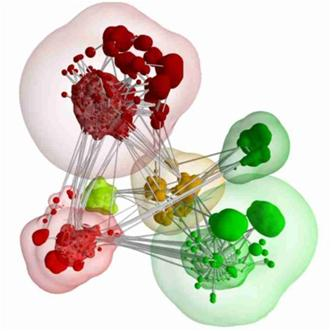
\includegraphics[scale=0.5]{../rapport/img/slide5.jpg}
      \end{figure}
    \end{column}
  \end{columns}
 \pause

  \begin{alertblock}{}
  \centering
    Impossibility for some nodes to move:
    node positions bring information
\end{alertblock}

\vspace{1cm}
} 

\frame{
  \frametitle{The context}
  \framesubtitle{Edge bundling}
  \begin{figure}[H]
    \centering
    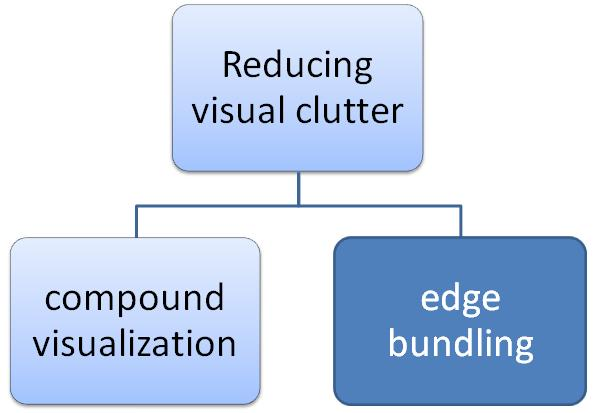
\includegraphics[scale=0.4]{../rapport/img/slide6.jpg}
  \end{figure}
 
\vspace{1cm}
} 

\frame{
  \frametitle{The context}
  \framesubtitle{Edge bundling}

\begin{alertblock}{}
  \centering
    Impossibility for some nodes to move:
    node positions bring information
\end{alertblock}
\pause
\begin{figure}[H]
        \centering
        
\includegraphics[scale=0.2]{../rapport/img/fleche.png}
      \end{figure}
\begin{center}
\begin{exampleblock}{}
\centering
Keep node position but edge aggregation
\end{exampleblock}
\end{center}                 
\pause 
 \begin{columns}[!ht]
\vspace{1cm}
    \begin{column}{6cm} 
    \begin{block}{}
    \centering
    Routes edges into bundles
    \end{block}
    \end{column}
    \begin{column}{6cm}   
      \begin{figure}[H]
        \centering
        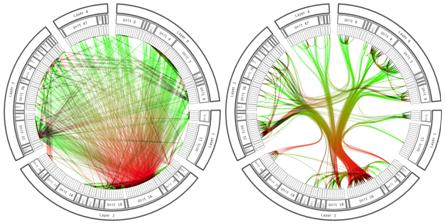
\includegraphics[scale=0.5]{../rapport/img/slide7_2.jpg}
      \end{figure}
    \end{column}
  \end{columns}

} 


\section{Tutte's theorem}
\subsection{Some extreme cases about Tutte's theorem}
In our project we do not use 3-connected graph but graph whose interior faces are triangle. It is obvious that considering the kind of graphs we used Tutte's theorem is verified because the fypothesis « All interior faces are tringle » is lighter than « 3-connected » hypothesis. So now we changed the hypothesis about the external polyhgon and the interior vertices in order to find out if the tutte's  is always verified.  

\subsubsection{Tutte's theorem and concave polygon}

In this section, we changed the hypothesis about the graph face. Now we consider a concave polygon face. Below is the illustration of a couterexample. 

\begin {figure}[H]
  \centering
  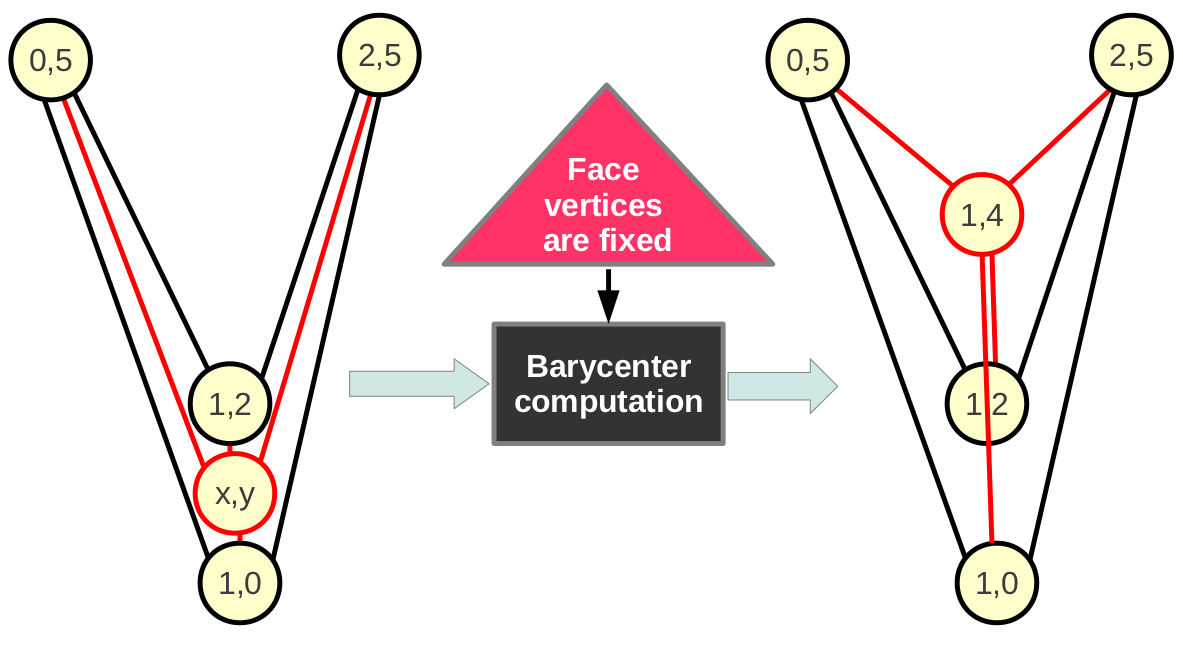
\includegraphics[scale=0.3]{img/tutte2.png}
  \caption{Tutte algorithm on concave polygon}
  \label{tutte2}
\end {figure}
\noindent
In the counterexample illustration above, the coordinate of the vertex shown in red color become $$(\frac{0+1+1+2}{4} , \frac{5+0+2+5}{4}) = (1 , 4)$$
One can see that after the the barycenter algorithm computation, the graph is no longer embedding. So the Tutte's theorem is not verified considering graphs with concave polygon face. 

\subsubsection{Tutte's algorithm and convex polygon with some fixed vertices}
This section kept the «convex polygon face» hypothesis but some internal vertices are considered fixed, their position never change during the barycenter algorithm computation. Below is the illustration of a couterexample. 

\begin {figure}[H]
  \centering
  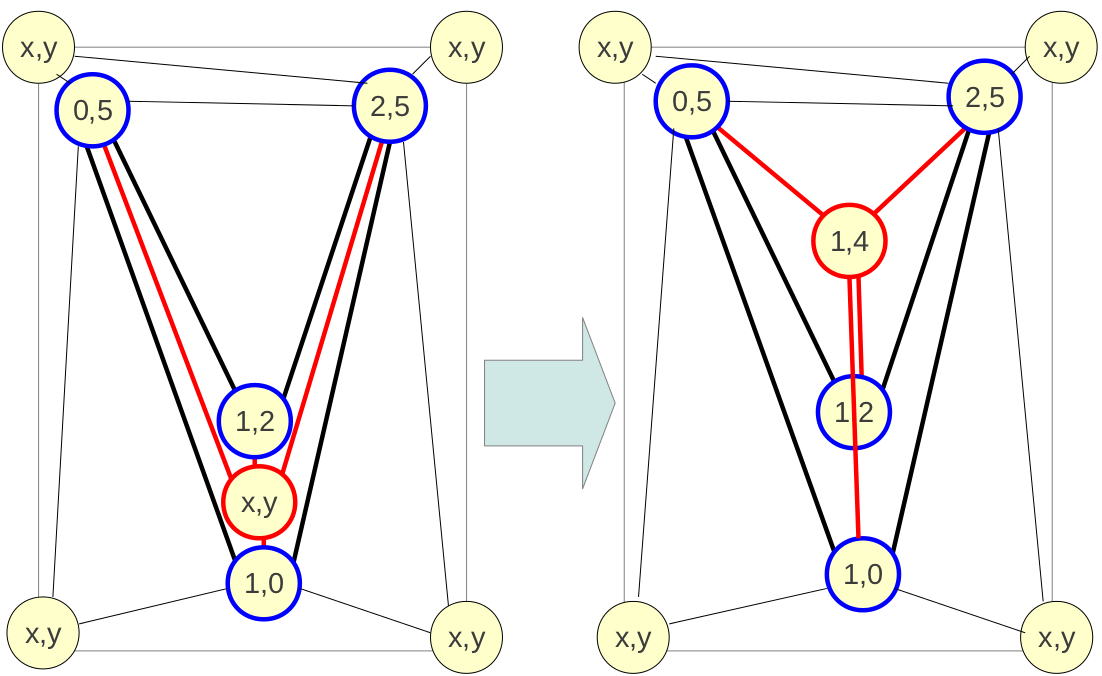
\includegraphics[scale=0.3]{img/tutte3.png}
  \caption{Tutte algorithm on convex polygon and fixes vertices}
  \label{tutte3}
\end {figure}
\noindent

As in the previous counterexample illustration (fig \ref{tutte2}) above, after the barycenter algorithm computation, the vertex shown in red color position changes. So the graph is no longer embedding which implies that the Tutte's theorem is not verified considering that some internal vertices can be fixed.


\section{Conclusion}
\chapter*{Conclusion}


With our best Tutte algorithm implementation , we obtain an algorithm convergence in 5 iterations and it spends x seconds to recalculate all the coordinates. (à mettre à jour)
Finally, our optimizations allowed an improvement of the clutter reduction and the performance compared with existent methods.


After discussing with our teachers in charge, some issues concerning our standalone version remains unresolved and could be taken into account in the future: Rather than working with input graph nodes, it would be interesting to dynamically add nodes (and their edges to keep a triangular-face graph) and launch again the algorithm in order to refine given results. It will also be quite interesting to automatically join small triangles or divide big triangles into littles ones. 

(à rajouter: plugin, prouver que ca marche: peut etre dû à la construction de la grille (triangulation de delaunay + contrainte: deux sommets fixes ne sont jamais reliés par une arête sauf sur le contour))

\end{document}
